\documentclass[11pt,letterpaper]{article}
\usepackage[utf8]{inputenc}
\usepackage[spanish,USenglish]{babel}
\usepackage{amsmath}
\usepackage{amsfonts}
\usepackage{amssymb}
\usepackage{amsthm}
\usepackage{graphicx}
\usepackage[left=2cm,right=2cm,top=2cm,bottom=2cm]{geometry}
\usepackage{flushend}
\usepackage{pgf,tikz, pgfplots}
\usetikzlibrary{arrows}
\pgfplotsset{compat=1.15}
\usepackage{pgf,tikz,pgfplots}
%escribir programas
\usepackage{listings}
\usepackage{algpseudocode}
\usepackage{algorithm}
\renewcommand{\algorithmicrequire}{\textbf{Input:}}
\renewcommand{\algorithmicensure}{\textbf{Output:}}

%encabezado
\usepackage{fancyhdr}
\pagestyle{fancy}
\fancyhf{}
\fancyhead[RO]{\thepage} % Números de página en las esquinas de los encabezados
%%%%%%%%%%%%%%%%%%%% BOXES %%%%%%%%%%%%%%%%%%%
\usepackage{bm}
\newcommand{\commentedbox}[2]{%
	\mbox{
		\begin{tabular}[t]{@{}c@{}}
			$\boxed{\displaystyle#1}$\\
			#2
		\end{tabular}%
	}%
}
\usepackage{framed}
\usepackage{wrapfig}\definecolor{shadecolor}{RGB}{224,238,238}
%%%%%%%%%%%%%%%%%%%%%%%%% DEFINITIONS %%%%%%%%%%%%%%%%%%%%%%%%
\theoremstyle{definition}
\newtheorem{defi}{Definición}[section]%Para definiciones
\theoremstyle{definition}
\newtheorem{teo}{Teorema}[section]%Para definiciones
\newtheorem{prop}{Proposición}
\theoremstyle{definition}
\newtheorem{ej}{Ejemplo}[section]
\newtheorem{lem}{Lema}
\newtheorem{prblm}{Problema}
\newtheorem{col}{Corolario}[section]



\title{\textbf{Tarea 8: Ajuste de Mezclas Gaussianas}\\ Optimización I \\ \Large {Maestría en Computación}\\ \Large {Centro de Investigación en Matemáticas}}
\author{Esteban Reyes Saldaña \\ esteban.reyes@citmat.mx}

\begin{document}

\selectlanguage{spanish}
\twocolumn[
\begin{@twocolumnfalse}
	\maketitle
	\centering\rule{0.9\textwidth}{0.1mm} 
	\begin{abstract}
		En esta tarea se realizó el ajuste de muestras Gaussianas de un histograma mediante la minimización con descenso gradiente. Dada la forma de la función a optimizar no se utilizaron métodos que necesitaran el Hessiano, en su lugar se usó búsqueda en línea con backtracking. Se presenta a continuación una descripción general, así como el pseudocódigo de los métodos implementados. Finalmente se incluyen conclusiones observadas a partir de la experimentación.
		\rule{0.9\textwidth}{0.1mm} 
	\end{abstract}
\end{@twocolumnfalse}]

\section{Introducción}
\subsection{Descenso Gradiente}
El objetivo general es encontrar los mínimos locales de una función $ f : \mathbb{R}^n \to \mathbb{R} $ tal que $ f(x) \in\mathcal{C}^1 $ de manera iterativa.
Un resultado muy conocido sobre el gradiente es
\begin{shaded*}
	\begin{teo}\label{max_}
		Sea $ f: \mathbb{R}^n \to \mathbb{R} $ una función continuamente diferenciable. Entonces la dirección donde $ f(x) $ crece más rápido es $ \nabla f(x) $.
	\end{teo}
\end{shaded*}

\begin{col}
	Bajo las condiciones del Teorema (\ref{max_}), $ f(x) $ decrece más rápido en la dirección $ - \nabla f(x) $.
\end{col}

\begin{shaded*}
	\begin{defi}
		Una \textbf{dirección de descenso} $ d \in \mathbb{R}^n $ para $ f \in \mathcal{C}^1 $ es un vector tal que
		\[ f(x + t d) < f(x) \]
		para $ t \in (0, T) $. Es decir, permite que el punto $ x $ más cerca al mínimo local $ x^* $ de la función objetivo $ f: \mathbb{R}^n \to \mathbb{R} $.
	\end{defi}
\end{shaded*}

\begin{shaded*}
	\begin{teo}
		Si $ g(x)^T d < 0 $ entonces $ d $ es una dirección de descenso.
	\end{teo}
\end{shaded*}


\subsection{Búsqueda en línea}
Este método usa la dirección $ d_k = - g(x_k) $ para moverse en cada iteración. El esquema general es
\begin{shaded*}
	\begin{enumerate}
	\item Dé un vector inicial $ x_0 $.
	\item Haga $ k = 0 $ y $ g_0 = \nabla f(x_0) $
	\item Mientras $ || g_k || \neq 0 $, 
	\begin{enumerate}
		\item $ \alpha_k = \displaystyle\arg \min_{\alpha >0} f(x_k - \alpha g_k) $
		\item $ x_{k+1} = x_k - \alpha_k g_k $
		\item $ g_{k+1} = \nabla f (x_{k+1}) $
		\item $ k \to k + 1 $
	\end{enumerate}
\end{enumerate}
\end{shaded*}
Se debe seleccionar un tamaño de paso $ \alpha_k $ tal que reduce suficientemente a $ f(x) $ y al mismo tiempo se requiere que sea eficiente.

\subsection{Condición de Armijo}
\begin{shaded*}
Un tamaño de decrecimiento suficiente se puede medir por la siguiente ecuación
\[  f(x_k + \alpha d_k) \leq f(x_k) + c_1 \alpha \nabla f_k^T d_k, \]
para alguna constante $ c_1 \in (0,1) $.
\end{shaded*}

\section{Método}
\subsection{Descripción del Problema}
Se utilizó el método de descenso de gradiente con búsqueda en línea \textbf{backtracking} para resolver el problema de ajustar una mezcla de guassianas a un histograma $ 3D $. La función objetivo de este problema viene dada por $\min_{\alpha^j, \mu^j} g (\alpha^j, \mu^j)$ donde
\begin{shaded*}
	\begin{equation}
		g (\alpha^j, \mu^j) = \sum_{ c \in \Omega} \left[ h^j (c) - \sum_{i = 1}^n \alpha_i^j \exp \left(- \dfrac{|| c - \mu_i^j ||_2^2}{2 \sigma^2} \right) \right]^2,
	\end{equation}
\end{shaded*}
donde 
\begin{itemize}
	\item $ j \in \{1,2\} $ corresponden a fondo y objeto.
	\item $ c = \left[ r, g, b \right]^T $, con $ r \in B_1 = \{ 1, \dots, b_1 \} $, \newline
	$ g \in B_2 = \{ 1, \dots, b_2 \} $, $ b \in B_3 = \{ 1, \dots, b_3 \} $ y $ b_1, b_2, b_3 $ son el número de bins en cada canal $ RGB $.
	\item $ \Omega = B_1 \times B_2 \times B_3 $, donde $ X \times Y := \{ (x,y) : x \in X, y \in Y \}$ representa el producto cartesiano.
	\item $ h^j (r, g,b) $ es el histograma $ 3D $ de la clase $ j $.
	\item $ n $ es el número de elementos en la base radial.
	\item $ \alpha^j = \left[ \alpha_1^j, \alpha_2^j, \dots, \alpha_n^j \right] $ son los pesos de la combinación lineal de la base radial.
	\item $ \mu^j = \left[ \mu_1^j, \mu_2^j, \dots, \mu_n^j \right] $ son las medias o posiciones de los elementos de la base radial.
	\item $ \sigma $ es un parámetro conocido.
\end{itemize}
El problema (1) se puede resolver de manera alternada hasta convergencia, es decir,
\begin{shaded*}
	\begin{eqnarray*}
		\alpha_{k+1}^j & = & \arg \min_{\alpha^j \in \mathbb{R}^n} g(\alpha^j, \mu_k ^j) \\
		\mu_{k+1}^j    & = & \arg \min_{\mu^j \in \mathbb{R}^n} g(\alpha^j_{k+1}, \mu^j)
	\end{eqnarray*}
\end{shaded*}
Para obtener los histogramas de clase se utilizó el programa \textit{histograma\_3D\_class.py} proporcionado por el Profesor.

\subsection{Gradiente de la función Objetivo}
Para implementar descenso con backtracking de manera iterativa se necesita calcular los gradientes de $ g(\alpha^j, \mu^j) $ respecto a $ \alpha^j $ y $ \mu^j $. Para manejar fácilmente las expresiones, sea
\begin{shaded*}
	\begin{equation*}
		w_k^j = \dfrac{|| c - \mu_k^j ||^2_2}{2 \sigma^2}
	\end{equation*}
\end{shaded*} 
\subsubsection{Gradiente respecto a $ \alpha^j $}
\footnotesize{
\begin{eqnarray*}
	\dfrac{\partial }{\partial \alpha_k^j} g(\alpha^j, \mu^j) 
	& = &
	2 \sum_{c\in \Omega} \left[ h^j (c) - \sum_{i = 1}^n \alpha_i^j \exp(w_i^j) \right] \\
	&   & \left[ - \dfrac{\partial }{\partial \alpha_k^j}
					\sum_{i = 1}^m \alpha_i^j \exp(-w_i^j) \right] \\
	& = &
	- 2 \sum_{c\in \Omega} \left[ h^j (c) - \sum_{i = 1}^n \alpha_i^j \exp(-w_i^j) \right]\\
	&   & \exp(-w_k^j)\\
\end{eqnarray*}
}
\normalsize{de donde}
\begin{shaded*}
	\footnotesize {\begin{equation}
		\dfrac{\partial }{\partial \alpha_k^j} g(\alpha^j, \mu^j) =
		- 2 \exp(-w_k^j) \sum_{c\in \Omega} \left[ h^j (c) - \sum_{i = 1}^n \alpha_i^j \exp(-w_i^j) \right]
	\end{equation}}
\end{shaded*}
\subsubsection{Gradiente respecto a $ \mu^j $}
\footnotesize{
	\begin{eqnarray*}
		\dfrac{\partial }{\partial \mu_k^j} g(\alpha^j, \mu^j) 
		& = &
		2 \sum_{c\in \Omega} \left[ h^j (c) - \sum_{i = 1}^n \alpha_i^j \exp(w_i^j) \right] \\
		&   & \left[ - \dfrac{\partial }{\partial \mu_k^j}
		\sum_{i = 1}^m \alpha_i^j \exp(-w_i^j) \right]
	\end{eqnarray*}
}

\normalsize{de donde}
\begin{shaded*}
\footnotesize {
	\begin{eqnarray*}
			\dfrac{\partial }{\partial \mu_k^j} g(\alpha^j, \mu^j) & = &
			- \dfrac{2}{\sigma^2} \sum_{c\in \Omega} \left[ h^j (c) - \sum_{i = 1}^n \alpha_i^j \exp(-w_i^j)
			 \right] \\
			 &  &
			\left[ \alpha_k^j \exp(w_k^j) (c - m_k^j) \right]
	\end{eqnarray*}
}
\end{shaded*}
\subsection{Pseudocódigo}
\subsubsection{Búsqueda con BackTracking}
\begin{shaded*}
	\begin{algorithmic}[1]
		% ENTRADA / SALIDA
		\Require{$ \hat{\alpha} $, $ \rho \in (0,1) $, $ c_1 \in (0,1) $}
		\Ensure{Tamaño de paso $ \alpha_k $}
		\State{Haga $ alpha = \hat{\alpha} $}
		\State{$inum =0 $}
		\While{$ f(x_k + \alpha d_k) > f(x_k) + c_1 \alpha \nabla f_k^T d_k $}
		\State{$ alpha \to \rho \alpha $}
		\EndWhile
		\State{Regresa $ \alpha_k = \alpha $}
	\end{algorithmic}
\end{shaded*}

\section{Resultados}
Para el método de \textbf{descenso gradiente} con  búsqueda en línea se usaron los parámetros
\begin{center}
	\begin{tabular}{cc}
		\hline
		Parámetro & Valor \\
		\hline
		$\alpha $ & 0.9 \\
		$ \rho $  & 0.5 \\
		$ c_1 $ & $ 10^{-4} $ \\
		\hline
	\end{tabular}
\end{center}

\begin{center}
	\begin{tabular}{ccccc}
		\hline
		Parámetro & $ max_{iter} $ & $ \tau_x $ & $ \tau_f $ & $ \tau_{grad} $ \\
		\hline
		 Valor    &      100     & $ 10^{-8} $ & $ 10^{-8} $ & $ 10^{-8} $  \\
		\hline
	\end{tabular}
\end{center}
Los valores para los vectores $ \alpha^j $ y $ \mu^j $ se generaron de manera aleatoria uniforme sobre $ [0, 1] $. Para realizar el ajuste gaussiano se eligieron
\begin{center}
	\begin{tabular}{ccccc}
		\hline
		Parámetro & $ nbins $ & $ radial_{size} $ & $ \sigma $ & $ max_{iter} $ \\
		\hline
		Valor    &      $ 3 $    & $ 10 $ & $ 0.5 $ & $ 500 $  \\
		\hline
	\end{tabular}
\end{center}
Se probó con tres imágenes del conjunto sugerido. A continuación se muestra la segmentación obtenida.
\begin{center}
	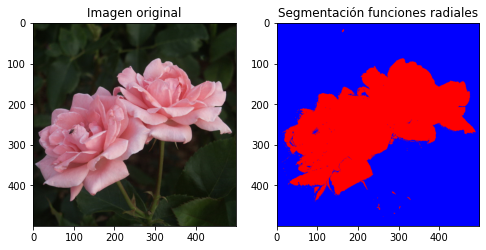
\includegraphics[width=0.7\linewidth]{graficas/rose_seg}
	\\
	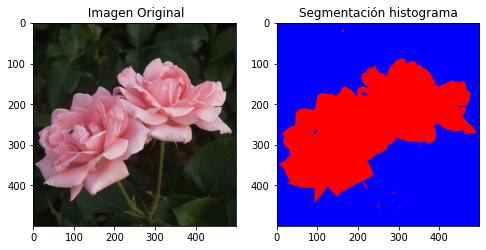
\includegraphics[width=0.7\linewidth]{graficas/rose_hist}
	\\
	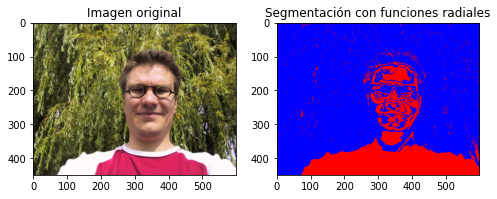
\includegraphics[width=0.7\linewidth]{graficas/person_seg}
	\\
	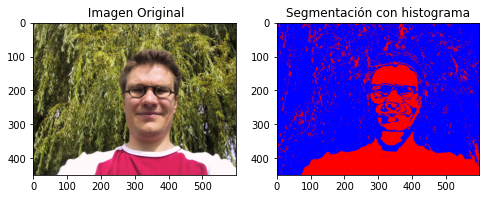
\includegraphics[width=0.7\linewidth]{graficas/person_hist}
	\\
	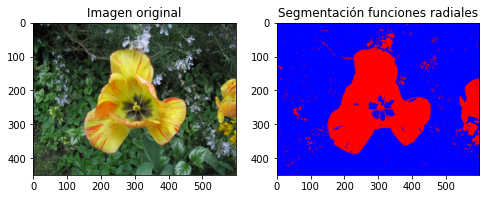
\includegraphics[width=0.7\linewidth]{graficas/flower_seg}
	\\
	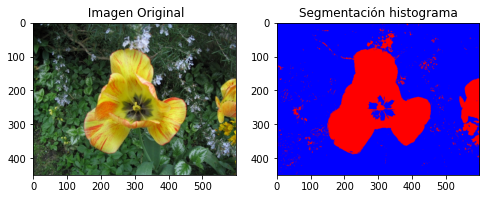
\includegraphics[width=0.7\linewidth]{graficas/flower_hist}
\end{center}
\section{Conclusiones}
	El problema de segmentación con bases Gaussianas se pudo resolver como un problema de optimización iterativa. De la experimentación de tareas previas se sabía que, comparado con algoritmos que utilizan el Hessiano de una función dada, suelen dar mejores resultados en cuando a tiempo de ejecución. Por lo anterior se le dieron solo $ 100 $ iteraciones al descenso gradiente. 
	\\
	Se observó también que la convergencia depende fuertemente de los valores iniciales para $ \alpha^j $, $ \mu^j $ y $ \sigma $.
	\\
	Además, la convergencia mejoró respecto al tiempo de ejecución para valores de $ \sigma $ cada vez más pequeños. Esto refleja la importancia de los valores $ w_k^j $, es decir, entre más pequeño el valor de $ \sigma $, más grande es la aportación de $ w_k^j $. Lo anterior también se refleja en los gradientes, por ejemplo, para el gradiente con respecto a $ \mu^j $, entre más pequeño es $ \sigma $, más grande es la norma del gradiente.

\end{document}